%% Copernicus Publications Manuscript Preparation Template for LaTeX Submissions
%% ---------------------------------
%% This template should be used for copernicus.cls
%% The class file and some style files are bundled in the Copernicus Latex Package, which can be downloaded from the different journal webpages.
%% For further assistance please contact Copernicus Publications at: production@copernicus.org
%% https://publications.copernicus.org/for_authors/manuscript_preparation.html


%% Please use the following documentclass and journal abbreviations for preprints and final revised papers.

%% 2-column papers and preprints
\documentclass[journal abbreviation, manuscript]{copernicus}

\def\MM#1{\boldsymbol{#1}}
\DeclareMathOperator{\diff}{d}
\newcommand{\avg}[1]{\{#1\}}
\newcommand{\jump}[1]{[\![#1]\!]}
\newcommand{\pp}[2]{\frac{\partial #1}{\partial #2}} 
\newcommand{\JScomment}[1]{\textit{\textbf{Jemma says: #1}}}

%% Journal abbreviations (please use the same for preprints and final revised papers)


% Advances in Geosciences (adgeo)
% Advances in Radio Science (ars)
% Advances in Science and Research (asr)
% Advances in Statistical Climatology, Meteorology and Oceanography (ascmo)
% Aerosol Research (ar)
% Annales Geophysicae (angeo)
% Archives Animal Breeding (aab)
% Atmospheric Chemistry and Physics (acp)
% Atmospheric Measurement Techniques (amt)
% Biogeosciences (bg)
% Climate of the Past (cp)
% DEUQUA Special Publications (deuquasp)
% Earth Surface Dynamics (esurf)
% Earth System Dynamics (esd)
% Earth System Science Data (essd)
% E&G Quaternary Science Journal (egqsj)
% EGUsphere (egusphere) | This is only for EGUsphere preprints submitted without relation to an EGU journal.
% European Journal of Mineralogy (ejm)
% Fossil Record (fr)
% Geochronology (gchron)
% Geographica Helvetica (gh)
% Geoscience Communication (gc)
% Geoscientific Instrumentation, Methods and Data Systems (gi)
% Geoscientific Model Development (gmd)
% History of Geo- and Space Sciences (hgss)
% Hydrology and Earth System Sciences (hess)
% Journal of Bone and Joint Infection (jbji)
% Journal of Micropalaeontology (jm)
% Journal of Sensors and Sensor Systems (jsss)
% Magnetic Resonance (mr)
% Mechanical Sciences (ms)
% Natural Hazards and Earth System Sciences (nhess)
% Nonlinear Processes in Geophysics (npg)
% Ocean Science (os)
% Polarforschung - Journal of the German Society for Polar Research (polf)
% Primate Biology (pb)
% Proceedings of the International Association of Hydrological Sciences (piahs)
% Safety of Nuclear Waste Disposal (sand)
% Scientific Drilling (sd)
% SOIL (soil)
% Solid Earth (se)
% State of the Planet (sp)
% The Cryosphere (tc)
% Weather and Climate Dynamics (wcd)
% Web Ecology (we)
% Wind Energy Science (wes)


%% \usepackage commands included in the copernicus.cls:
%\usepackage[german, english]{babel}
%\usepackage{tabularx}
%\usepackage{cancel}
%\usepackage{multirow}
%\usepackage{supertabular}
%\usepackage{algorithmic}
%\usepackage{algorithm}
%\usepackage{amsthm}
%\usepackage{float}
%\usepackage{subfig}
%\usepackage{rotating}

\begin{document}

\title{Gusto: a toolkit for compatible finite element dynamical cores}

% \Author[affil]{given_name}{surname}

\Author[1,*]{Jemma}{Shipton}
\Author[2]{Thomas M.}{Bendall}
\Author[3]{So many}{Others}

\affil[1]{Department of Mathematics and Statistics, University of Exeter}
\affil[2]{Met Office}

%% The [] brackets identify the author with the corresponding affiliation. 1, 2, 3, etc. should be inserted.

%% If an author is deceased, please mark the respective author name(s) with a dagger, e.g. "\Author[2,$\dag$]{Anton}{Smith}", and add a further "\affil[$\dag$]{deceased, 1 July 2019}".

%% If authors contributed equally, please mark the respective author names with an asterisk, e.g. "\Author[2,*]{Anton}{Smith}" and "\Author[3,*]{Bradley}{Miller}" and add a further affiliation: "\affil[*]{These authors contributed equally to this work.}".


\correspondence{NAME (EMAIL)}

\runningtitle{TEXT}

\runningauthor{TEXT}





\received{}
\pubdiscuss{} %% only important for two-stage journals
\revised{}
\accepted{}
\published{}

%% These dates will be inserted by Copernicus Publications during the typesetting process.


\firstpage{1}

\maketitle



\begin{abstract}
TEXT
\end{abstract}

\begin{itemize}
\item Section 1: why compatible FEM
\item Section 2: why Gusto
\item Sections 3 and 4: this is Gusto
\item Section 5: and here are some examples of what we can currently do
\end{itemize}

\introduction   %% \introduction[modified heading if necessary]

\subsection{Motivation}
\begin{itemize}
\item many choices and research to be done - Colin says so in his Acta Numerica paper! - therefore flexible implementation is useful
\end{itemize}

Compatible finite elements provide a route to stable, consistent
discretisations of the partial differential equations governing
geophysical fluids which also have the correct wave propagation speeds
and avoid spurious computational modes, even on non-uniform
grids. These properties, along with conservation of mass and
potentially other quantities such as energy and enstrophy, are
considered essential for the accuracy of the dynamical core of weather
and climate models \citep{staniforth2012horizontal}. Achieving these
properties on a non-orthogonal grid is important because of parallel
scaling**. While the required properties of the discretisation guide the
choice of finite element spaces, there are many options for both the
spatial and temporal discretisation and it is not clear which will be
best for any particular problem. Gusto provides a flexible,
extensible, easy-to-use toolkit of options for rapid prototyping of
different spatial and temporal discretisations based on the compatible
finite element framework applied to geophysical fluid dynamics
equations relevant to numerical weather and climate prediction. In
this paper we introduce Gusto to the community, summarise its current
capabilities and outline our vision for future development.

\subsection{Background}

\begin{itemize}
\item overall theory is described in \citet{gibson2019compatible, cotter2023compatible}
\item Gusto has grown out of code described in \citet{natale2016compatible, cotter2012mixed, bendall2019recovered, bendall2020compatible, yamazaki2017vertical, shipton2018higher}
\item links to LFRic - we mention the Gung Ho project on the Gusto website so should describe that link here
\end{itemize}

The finite element method represents fields on a mesh made of
non-overlapping, conforming cells, or elements. Within each element,
the field is represented as a sum of coefficients multiplied by
polynomial basis functions. The finite element space is specified by
the degree of the polynomial basis functions and the continuity of
these functions between the elements. The partial differential
equations used in weather and climate modelling have multiple
prognostic fields and it is not necessary, or indeed desirable, to use
the same finite element function space for each field. Using different
finite element function spaces for each field gives what is known as a
mixed finite element discretisation. If these different finite element
function spaces are chosen so that discrete versions of the vector
calculus identities ** hold then the discretisation is called
`mimetic' or `compatible'.

In this article we will describe the current capabilities of Gusto and
the design features that enable our flexible implementation whereby
different spatial and temporal discretisations can be applied to a
range of different equation sets relevant for weather and climate
modelling. In section \ref{sec: governing} we will outline three
different equation sets, along with their finite element
discretisations. Then in section \ref{sec: design} we will present the
code structure of Gusto followed by a detailed example (section
\ref{sec: FML}) of the Form Manipulation Language (FML) that facilitates
symbolic manipulation of the finite element forms within our
timestepping code. Section \ref{sec: results} contains a selection of
numerical results that showcases the range of discretisations
available within Gusto. We summarise our current status and future
directions in section \ref{sec: summary}.

\section{Governing Equations}
\label{sec: governing}
The aim of this section is to introduce three governing equation sets
commonly used in the development of weather and climate models, along
with enough detail about the finite element discretiations provided by
Gusto to demonstrate the similarities between them. These similarities
guide the design of the code structure described in the next section
and motivate the use of Form Manipulation Labelling (FML) that
underlies the flexibility of Gusto, a detailed example of which will
be given in section \ref{sec: FML}. The convention in Gusto is to
write the equations in residual form, meaning that all the terms
appear on the left hand side. We will follow this convention below in
contrast to many papers which present the equations with the pressure
gradient term and any forcing terms on the right hand side.

\subsection{Shallow Water Equations}
The shallow water equations are commonly used for testing numerical
algorithms and for exploring geophysical fluid dynamics concepts under
simplified conditions. They are useful in both contexts since they are
the simplest set of equations that model motion on both the slow,
geostrophic timescale and the much faster timescale of the
inertia-gravity waves. This timescale separation poses challenges to
the numerical discretisation and also provides a rich enough range of
dynamics to explain many of the phenomena observed in the atmosphere
and oceans \citep{zeitlin2018geophysical}.

The shallow water equations describe the flow of a shallow layer of
fluid subject to gravitational and, optionally, rotational forces. The
prognostic variables are the two horizontal velocity components
$\MM{u} = (u, v)$ and the fluid depth $D = H + h - b$ where $H$ is the
undisturbed depth of the fluid layer, $h$ is the perturbation to the
fluid depth and $b$ is the bottom topography, if present. The
equations are:

\begin{align}
  \pp{\MM{u}}{t} + \MM{u}\cdot\nabla\MM{u} + f\hat{\MM{k}}\times\MM{u} + g\nabla (D+b) &= 0, \\
  \pp{D}{t} + \nabla\cdot(D\MM{u}) &= 0,
\end{align}
where $f$ is the Coriolis parameter, $\hat{\MM{k}}$ is the unit vector
pointing upwards and $g$ is the acceleration due to gravity. The
nonlinear velocity advection term can be replaced by the sum of a
vorticity-based term and the gradient of the kinetic energy. This is
known as the vector invariant form and it enables the construction of
schemes that conservation energy and/or enstrophy
\citep{mcrae2014energy, bauer2018energy, wimmer2020energy,
  wimmer2021energy}. However, this form can exhibit numerical
instabilities \citep{bell2017numerical} and it is not yet clear which
form is preferable so in Gusto we offer both forms of the equations.

\subsection{Compressible Boussinesq Equations}
The compressible Boussinesq equations are commonly used in ocean
modelling. They are useful from a numerical discretisation perspective
because they incorporate compressibility effects without the
complexity of discretising the nonlinear pressure gradient terms that
we shall see in the compressible Euler equations. We write these
equations in terms of the prognostic variables $\MM{u}$, $b$ and
$p$ where $\MM{u}=(u, v, w)$ is now a three dimensional velocity
field, $b$ is the fluid buoyancy and $p$ is pressure. In terms of
these variables, the equations are:

\begin{align}
  \pp{\MM{u}}{t} + 
  (\MM{u}\cdot\nabla)\MM{u} +
  2\MM{\Omega}\times \MM{u} + \nabla p + b\hat{\MM{k}} & = 0, \\
  \pp{p}{t} + c^2\nabla\cdot\MM{u} & = 0, \\
  \pp{b}{t} + \MM{u}\cdot\nabla b & = 0,
\end{align}
where $\MM{\Omega}$ is the rotation vector of the domain,
$\hat{\MM{k}}$ is the unit vector pointing upwards and $c$ is the
acoustic wave speed.

\subsection{Compressible Euler Equations}
The dynamical core at the heart of any weather or climate model solves
the rotating compressible Euler equations that model atmospheric
flow. We write these equations in terms of the prognostic variables
$\MM{u}$, $\rho$ and $\theta$ where $\MM{u}=(u, v, w)$ is now a three
dimensional velocity field, $\rho$ is the fluid density and $\theta$
is the potential temperature. The pressure gradient term is written in
terms of the Exner pressure $\Pi$ which is calculated through an
equation of state. In terms of these variables, the equations are:

\begin{align}
  \pp{\MM{u}}{t} + 
  (\MM{u}\cdot\nabla)\MM{u} +
  2\MM{\Omega}\times \MM{u} + c_p\theta\nabla \Pi + g\hat{\MM{k}} & = 0, \\
  \pp{\rho}{t} + \nabla\cdot(\MM{u}\rho) & = 0, \\
  \pp{\theta}{t} + \MM{u}\cdot\nabla\theta & = 0, \\
  \Pi^{(1-\kappa)/\kappa} & = \frac{R}{p_0}\rho\theta, & 
\end{align}
where $\Pi$ is the Exner pressure, $p_0$ is a reference pressure,
typically taken to be *, $R$ is ** and $\kappa$ is **.

\section{Finite Element Discretisation}
\label{sec: FEM}

Comparing the equation sets given in the previous sections, we see
several similarities. For example, the prognostic equation for the
velocity always contains a nonlinear transport term, a term due to
rotation and a `pressure' gradient term (in shallow water this is the
gradient of the depth but the term plays the same role in the dynamics
and is derived from the pressure gradient term in the full equations
(**cite Zeitlin book)). The other prognostic fields satisfy either an
advective or continuity form of the transport equation. These
similarities remain when we formulate the compatible finite element
discretisations, as we shall see below, and importantly this means
that the discretisation of these terms can be written in a general way
that means it can be applied to any of the equation sets.

The finite element discretisation is formed by choosing appropriate
function spaces for the prognostic variables, multiplying by test
functions from these function spaces and integrating over the
domain. In addition to this, we integrate by parts when the
inter-element continuity of the basis functions is not sufficient to
define the result of applying the differential operator directly.

In line with the theory outlined in section \ref{}, we always choose
the velocity $\MM{u} \in \mathbb{V}_u$ with $\mathbb{V}_u \subset
H(\text{div})$. The field whose gradient appears in the `pressure'
gradient term is chosen to be in the space $\mathbb{V}_p$ with
$\mathbb{V}_p \subset L_2$. The compressible Boussinesq and
compressible Euler equations have a third prognostic variable, either
buoyancy or potential temperature, which is chosen to be in the space
$\mathbb{V}_\theta$ which has degrees of freedom that are collocated
with those of the vertical velocity, mimicking the Charney-Phillips
staggering as discussed in **. These choices are governed by the
properties required of discretisation of the linearised equation sets
(as discussed in section ** and other refs). To solve the nonlinear
equation sets we need to introduce stable and accurate discretisations
of the transport terms and the nonlinear pressure gradient term in the
compressible Euler equation set. In addition, some test cases require
the addition of viscous and diffusive terms to generate converged
solutions \ref{}. In the following subsections we illustrate a
non-exhaustive (**probably!) selection of the options available in
Gusto.

\subsection{Transport terms}
Since the prognostic variables are discretised using different finite
element function spaces $\mathbb{V}_u$, $\mathbb{V}_p$ and
$\mathbb{V}_\theta$, each with different continuity properties between
the elements, the choice of stable transport discretisation is
different for each prognostic variable. 


\subsection{Pressure gradient term}
The pressure gradient term is discretised in a similar way for each
equation set, with some additional considerations required for the
nonlinear form of this term in the compressible Euler equations. Since
the pressure (or depth, for shallow water) field is discretised in
$\mathbb{V}_p \subset L_2$, the gradient is not defined globally and
the term must be integrated by parts. In the linear case, using the
notation for the compressible Boussinesq equations, the weak form is

\begin{equation}
\int_\Omega\MM{w}\cdot\nabla p \diff x = -\int_\Omega\nabla\cdot\MM{w}p\diff x,
\end{equation}
where $\Omega$ denotes the domain and there are no surface terms from
the integration by parts because these vanish on interior element
boundaries since the normal component of $\MM{w}$ is continuous across
element faces and on exterior boundaries we set no normal flow
boundary conditions. However, the pressure gradient term in the
compressible Euler equations, $c_p\theta\nabla\Pi$, is nonlinear and
this introduces an additional complication. Integrating by parts is
still required since $\Pi$ is evaluated as a function of the density
$\rho \in L_2$ and so is discontinuous, but this means that we now
have a differential operator applied to $\theta \in \mathbb{V}_\theta$
which is discontinuous in the vertical. Following \ref{} we integrate
by parts in each element $e$, giving

\begin{equation}
  c_p\int_e\MM{w}\cdot\theta\nabla\Pi\diff x = -c_p\int_e\nabla\cdot(\MM{w}\theta)\Pi\diff x + c_p\int_{\partial e}\theta^-\MM{w}\cdot\MM{n}\Pi^- \diff S,
\end{equation}
where $\partial e$ denotes the element faces, $\MM{n}$ is the outward
pointing normal to the face and $\cdot^-$ denotes the value of a
variable on the interior side of the boundary. Summing over the domain
gives

\begin{equation}
  c_p\int_\Omega\MM{w}\cdot\theta\nabla\Pi\diff x = -c_p\int_\Omega\nabla\cdot(\MM{w}\theta)\Pi\diff x + c_p\int_{\Gamma_v}\jump{\theta\MM{w}\cdot\MM{n}}\avg{\Pi} \diff S,
\end{equation}
where $\jump{\cdot}$ and $\avg{\cdot}$.

\subsection{Viscous and diffusive terms}

** Don't do whole equation set - go term by term and try to write as
few equations as possible: transport, pressure gradient, diffusion


\section{Software Design}
\label{sec: design}
Gusto is built on top of the Firedrake package, an automated system
for solving partial differential equations using the finite element
method. This gives many advantages, not least that it provides the
finite element machinery required to translate the discretisations
written in the previous section in to the matrix-vector equations that
we need to solve. This is done using the Unified Form Language (UFL),
a domain specific language that enables the definition of the finite
element forms within Python. The other packages that Firedrake depends
on are summarised in \citet{davies2022towards} but we note that we
make particular use of higher order mesh representation on curved
manifolds (**ref), extruded meshes (**ref) and the PETSc library
solver options (**ref).

\begin{figure}
  \centering{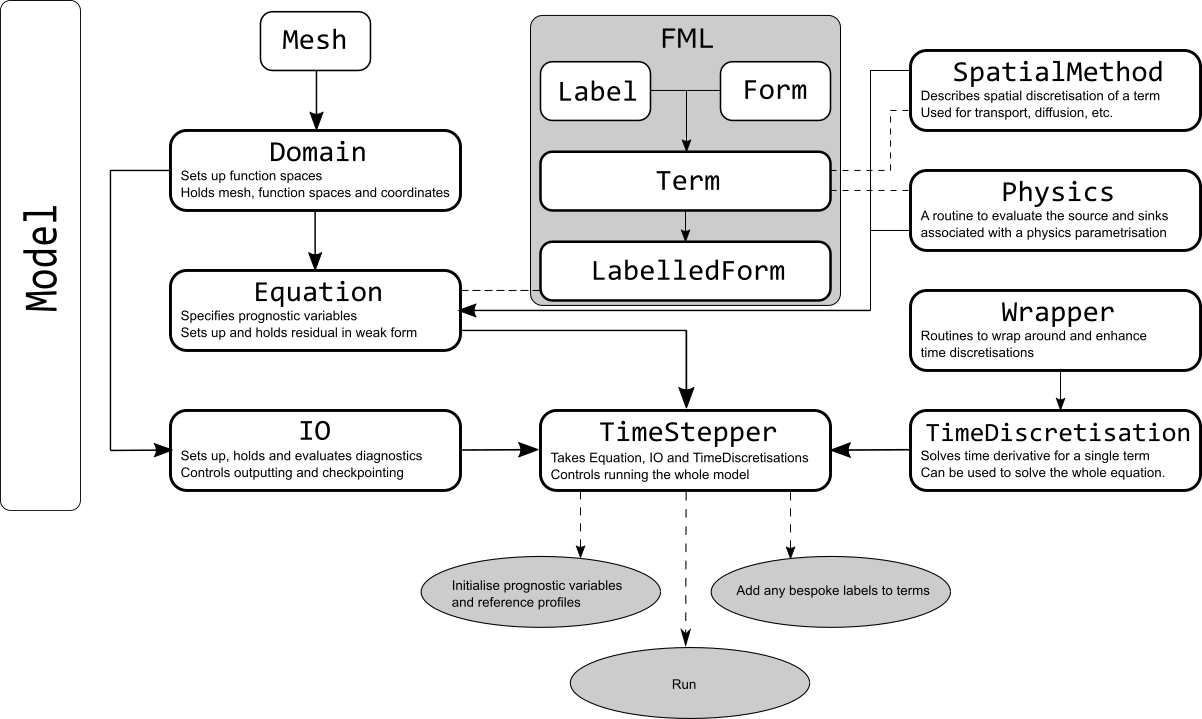
\includegraphics[width=0.8\textwidth]{gusto_schematic.png}}
\end{figure}

\JScomment{Text here depends on what the schematic looks like - this
  paragraph should refer to the schematic and explain all aspects} The
Gusto model comprises a domain and a prognostic equation set. The
domain holds the mesh and the finite element function spaces along
with any other information about the space-time domain such as the
coordinates and the timestep. The Prognostic equation sets are each
defined in a python class, making use of the common finite element
forms for the transport and difffusion terms. The timeloop class
contains the definition of the timestepping procedure and the
\texttt{run} method that loops over the timesteps. It also sets up
diagnostic fields and calls the IO as required. The simplest timeloop
class will just apply one time discretisation method to the equation
set but it is common in weather and climate prediction models to split
the different types of terms and apply a time discretisation
separately to each type of term. For example, the transport and
forcing terms might be solved for separately, such as in **, which
enables explicit transport schemes to be applied to each field. **
something about SIQN structure. Terms related to the physics are
solved for in the appropriate part of the iteration loop, with physics
processes that occur on `fast' timescales evaluated more frequently
and `slower' physics processes evaluated just once at the end of the
timestep. The choice of where to evaluate the physics processes in the
iteration is also based on the computational cost and the best way to
do this is still an open research question (**ref).

\begin{itemize}
\item include schematic
\item generic example - no FML
\item lead in to next section... facilitated by FML i.e. timesteppers don't care what equations they're given because forms are labelled
\end{itemize}

\section{Form Manipulation Language}
\label{sec: FML}
The discussion of the time discretisation so far has been general i.e.
not specific to any particular equation set. This is also true of the
implementation of the timestepping schemes. This enables flexibility
and reproducibility (**elaborate). This functionality is enabled
through the form manipulation language (FML) which is used to
associate a label to each term in the residual form defined in the
equation class. The timestepping methods are then able to reason about
which manipulations to apply to which forms by applying filters. A
simple example would be a splitting method that evaluates transport
terms and diffusion terms separately. The full residual is passed to
the transport scheme which then applies a filter to drop all terms
that are not labelled as transport; similarly for diffusion. We
illustrate this procedure in figure \ref{fig:advdiff} where we show
the definition of the residual for the advection diffusion equation
for a scalar variable $q$ with a prescribed transport velocity
$\MM{c}$ and diffusivity $\kappa$

\begin{equation}
  q_t + \MM{c}\cdot\nabla q - \kappa\nabla^2 q = 0,
\end{equation}
with the terms labelled either \texttt{time\_derivative},
\texttt{transport} or \texttt{diffusion}. The timestepping loop then
applies a step of forward Euler to the transport term and backwards
Euler to the diffusive term, i.e. the time discretisation is

\begin{align}
  q^* &= q^n - \Delta t (\MM{c}\cdot\nabla) q^n, \\
  q^{n+1} &= q^* + \Delta t \kappa \nabla^2 q^{n+1}.
\end{align}



\section{Results}
\label{sec: results}
The aim of this section is to present a selection of results that
demonstrate the tools available in Gusto, such as the choice of grids,
HDiv element families, order of finite element spaces, different
spatial discretisation options, timestepping schemes and physics. The
numerical properties of these configurations (convergence, stability,
accuracy and efficiency) have either been demonstrated elsewhere, or
will be investigated more thoroughly in future publications.

To include:
\begin{itemize}
\item terminator toy (Tim)
\item shallow water on different grids and with different HDiv
  families (Nell) e.g. Williamson 5 cubed sphere PV and Galewsky
  icosahedral sphere PV, high res (ref 6)
\item convergence with different RK schemes / multistage schemes using
  Williamson 2 or 6, L2 and Linf errors for D and u (2 plots, one L2,
  one Linf) (Alex)
\item vertical slice Euler - Straka, different orders, illustrates
  recovery for diffusion (Tom)
\item 3D moist bubble with rain (Tom/Alex)
\item spherical gravity wave, Boussinesq (Jemma)
\item spherical baroclinic wave, Euler - whatever people usually plot
  (horizontal slice pressure contours, temperature shadng) (Dan)
\item Held Suarez??
\end{itemize}

\subsection{Shallow water simulations}
The standard suite of shallow water test cases originally proposed in
\citet{williamson1992standard} provides a common starting point for
testing new discretisations. This test suite is usually augmented by
the unstable barotropic jet described in \citet{galewsky2004initial}
(**and linear tests?)





\section{Summary}
\label{sec: summary}


\conclusions  %% \conclusions[modified heading if necessary]
TEXT

%% The following commands are for the statements about the availability of data sets and/or software code corresponding to the manuscript.
%% It is strongly recommended to make use of these sections in case data sets and/or software code have been part of your research the article is based on.

\codeavailability{TEXT} %% use this section when having only software code available


\dataavailability{TEXT} %% use this section when having only data sets available


\codedataavailability{TEXT} %% use this section when having data sets and software code available


\sampleavailability{TEXT} %% use this section when having geoscientific samples available


\videosupplement{TEXT} %% use this section when having video supplements available


\appendix
\section{}    %% Appendix A

\subsection{}     %% Appendix A1, A2, etc.


\noappendix       %% use this to mark the end of the appendix section. Otherwise the figures might be numbered incorrectly (e.g. 10 instead of 1).

%% Regarding figures and tables in appendices, the following two options are possible depending on your general handling of figures and tables in the manuscript environment:

%% Option 1: If you sorted all figures and tables into the sections of the text, please also sort the appendix figures and appendix tables into the respective appendix sections.
%% They will be correctly named automatically.

%% Option 2: If you put all figures after the reference list, please insert appendix tables and figures after the normal tables and figures.
%% To rename them correctly to A1, A2, etc., please add the following commands in front of them:

\appendixfigures  %% needs to be added in front of appendix figures

\appendixtables   %% needs to be added in front of appendix tables

%% Please add \clearpage between each table and/or figure. Further guidelines on figures and tables can be found below.



\authorcontribution{TEXT} %% this section is mandatory

\competinginterests{TEXT} %% this section is mandatory even if you declare that no competing interests are present

\disclaimer{TEXT} %% optional section

\begin{acknowledgements}
TEXT
\end{acknowledgements}




%% REFERENCES

%% The reference list is compiled as follows:

%% \begin{thebibliography}{}

%% \bibitem[AUTHOR(YEAR)]{LABEL1}
%% REFERENCE 1

%% \bibitem[AUTHOR(YEAR)]{LABEL2}
%% REFERENCE 2

%% \end{thebibliography}

%% Since the Copernicus LaTeX package includes the BibTeX style file copernicus.bst,
%% authors experienced with BibTeX only have to include the following two lines:
%%
\bibliographystyle{copernicus}
\bibliography{references.bib}
%%
%% URLs and DOIs can be entered in your BibTeX file as:
%%
%% URL = {http://www.xyz.org/~jones/idx_g.htm}
%% DOI = {10.5194/xyz}


%% LITERATURE CITATIONS
%%
%% command                        & example result
%% \citet{jones90}|               & Jones et al. (1990)
%% \citep{jones90}|               & (Jones et al., 1990)
%% \citep{jones90,jones93}|       & (Jones et al., 1990, 1993)
%% \citep[p.~32]{jones90}|        & (Jones et al., 1990, p.~32)
%% \citep[e.g.,][]{jones90}|      & (e.g., Jones et al., 1990)
%% \citep[e.g.,][p.~32]{jones90}| & (e.g., Jones et al., 1990, p.~32)
%% \citeauthor{jones90}|          & Jones et al.
%% \citeyear{jones90}|            & 1990



%% FIGURES

%% When figures and tables are placed at the end of the MS (article in one-column style), please add \clearpage
%% between bibliography and first table and/or figure as well as between each table and/or figure.

% The figure files should be labelled correctly with Arabic numerals (e.g. fig01.jpg, fig02.png).


%% ONE-COLUMN FIGURES

%%f
%\begin{figure}[t]
%\includegraphics[width=8.3cm]{FILE NAME}
%\caption{TEXT}
%\end{figure}
%
%%% TWO-COLUMN FIGURES
%
%%f
%\begin{figure*}[t]
%\includegraphics[width=12cm]{FILE NAME}
%\caption{TEXT}
%\end{figure*}
%
%
%%% TABLES
%%%
%%% The different columns must be seperated with a & command and should
%%% end with \\ to identify the column brake.
%
%%% ONE-COLUMN TABLE
%
%%t
%\begin{table}[t]
%\caption{TEXT}
%\begin{tabular}{column = lcr}
%\tophline
%
%\middlehline
%
%\bottomhline
%\end{tabular}
%\belowtable{} % Table Footnotes
%\end{table}
%
%%% TWO-COLUMN TABLE
%
%%t
%\begin{table*}[t]
%\caption{TEXT}
%\begin{tabular}{column = lcr}
%\tophline
%
%\middlehline
%
%\bottomhline
%\end{tabular}
%\belowtable{} % Table Footnotes
%\end{table*}
%
%%% LANDSCAPE TABLE
%
%%t
%\begin{sidewaystable*}[t]
%\caption{TEXT}
%\begin{tabular}{column = lcr}
%\tophline
%
%\middlehline
%
%\bottomhline
%\end{tabular}
%\belowtable{} % Table Footnotes
%\end{sidewaystable*}
%
%
%%% MATHEMATICAL EXPRESSIONS
%
%%% All papers typeset by Copernicus Publications follow the math typesetting regulations
%%% given by the IUPAC Green Book (IUPAC: Quantities, Units and Symbols in Physical Chemistry,
%%% 2nd Edn., Blackwell Science, available at: http://old.iupac.org/publications/books/gbook/green_book_2ed.pdf, 1993).
%%%
%%% Physical quantities/variables are typeset in italic font (t for time, T for Temperature)
%%% Indices which are not defined are typeset in italic font (x, y, z, a, b, c)
%%% Items/objects which are defined are typeset in roman font (Car A, Car B)
%%% Descriptions/specifications which are defined by itself are typeset in roman font (abs, rel, ref, tot, net, ice)
%%% Abbreviations from 2 letters are typeset in roman font (RH, LAI)
%%% Vectors are identified in bold italic font using \vec{x}
%%% Matrices are identified in bold roman font
%%% Multiplication signs are typeset using the LaTeX commands \times (for vector products, grids, and exponential notations) or \cdot
%%% The character * should not be applied as mutliplication sign
%
%
%%% EQUATIONS
%
%%% Single-row equation
%
%\begin{equation}
%
%\end{equation}
%
%%% Multiline equation
%
%\begin{align}
%& 3 + 5 = 8\\
%& 3 + 5 = 8\\
%& 3 + 5 = 8
%\end{align}
%
%
%%% MATRICES
%
%\begin{matrix}
%x & y & z\\
%x & y & z\\
%x & y & z\\
%\end{matrix}
%
%
%%% ALGORITHM
%
%\begin{algorithm}
%\caption{...}
%\label{a1}
%\begin{algorithmic}
%...
%\end{algorithmic}
%\end{algorithm}
%
%
%%% CHEMICAL FORMULAS AND REACTIONS
%
%%% For formulas embedded in the text, please use \chem{}
%
%%% The reaction environment creates labels including the letter R, i.e. (R1), (R2), etc.
%
%\begin{reaction}
%%% \rightarrow should be used for normal (one-way) chemical reactions
%%% \rightleftharpoons should be used for equilibria
%%% \leftrightarrow should be used for resonance structures
%\end{reaction}
%
%
%%% PHYSICAL UNITS
%%%
%%% Please use \unit{} and apply the exponential notation


\end{document}
